\section{Control Structures}

%didn't work at all, write by hand
\section*{Branch Instructions}
\begin{center}
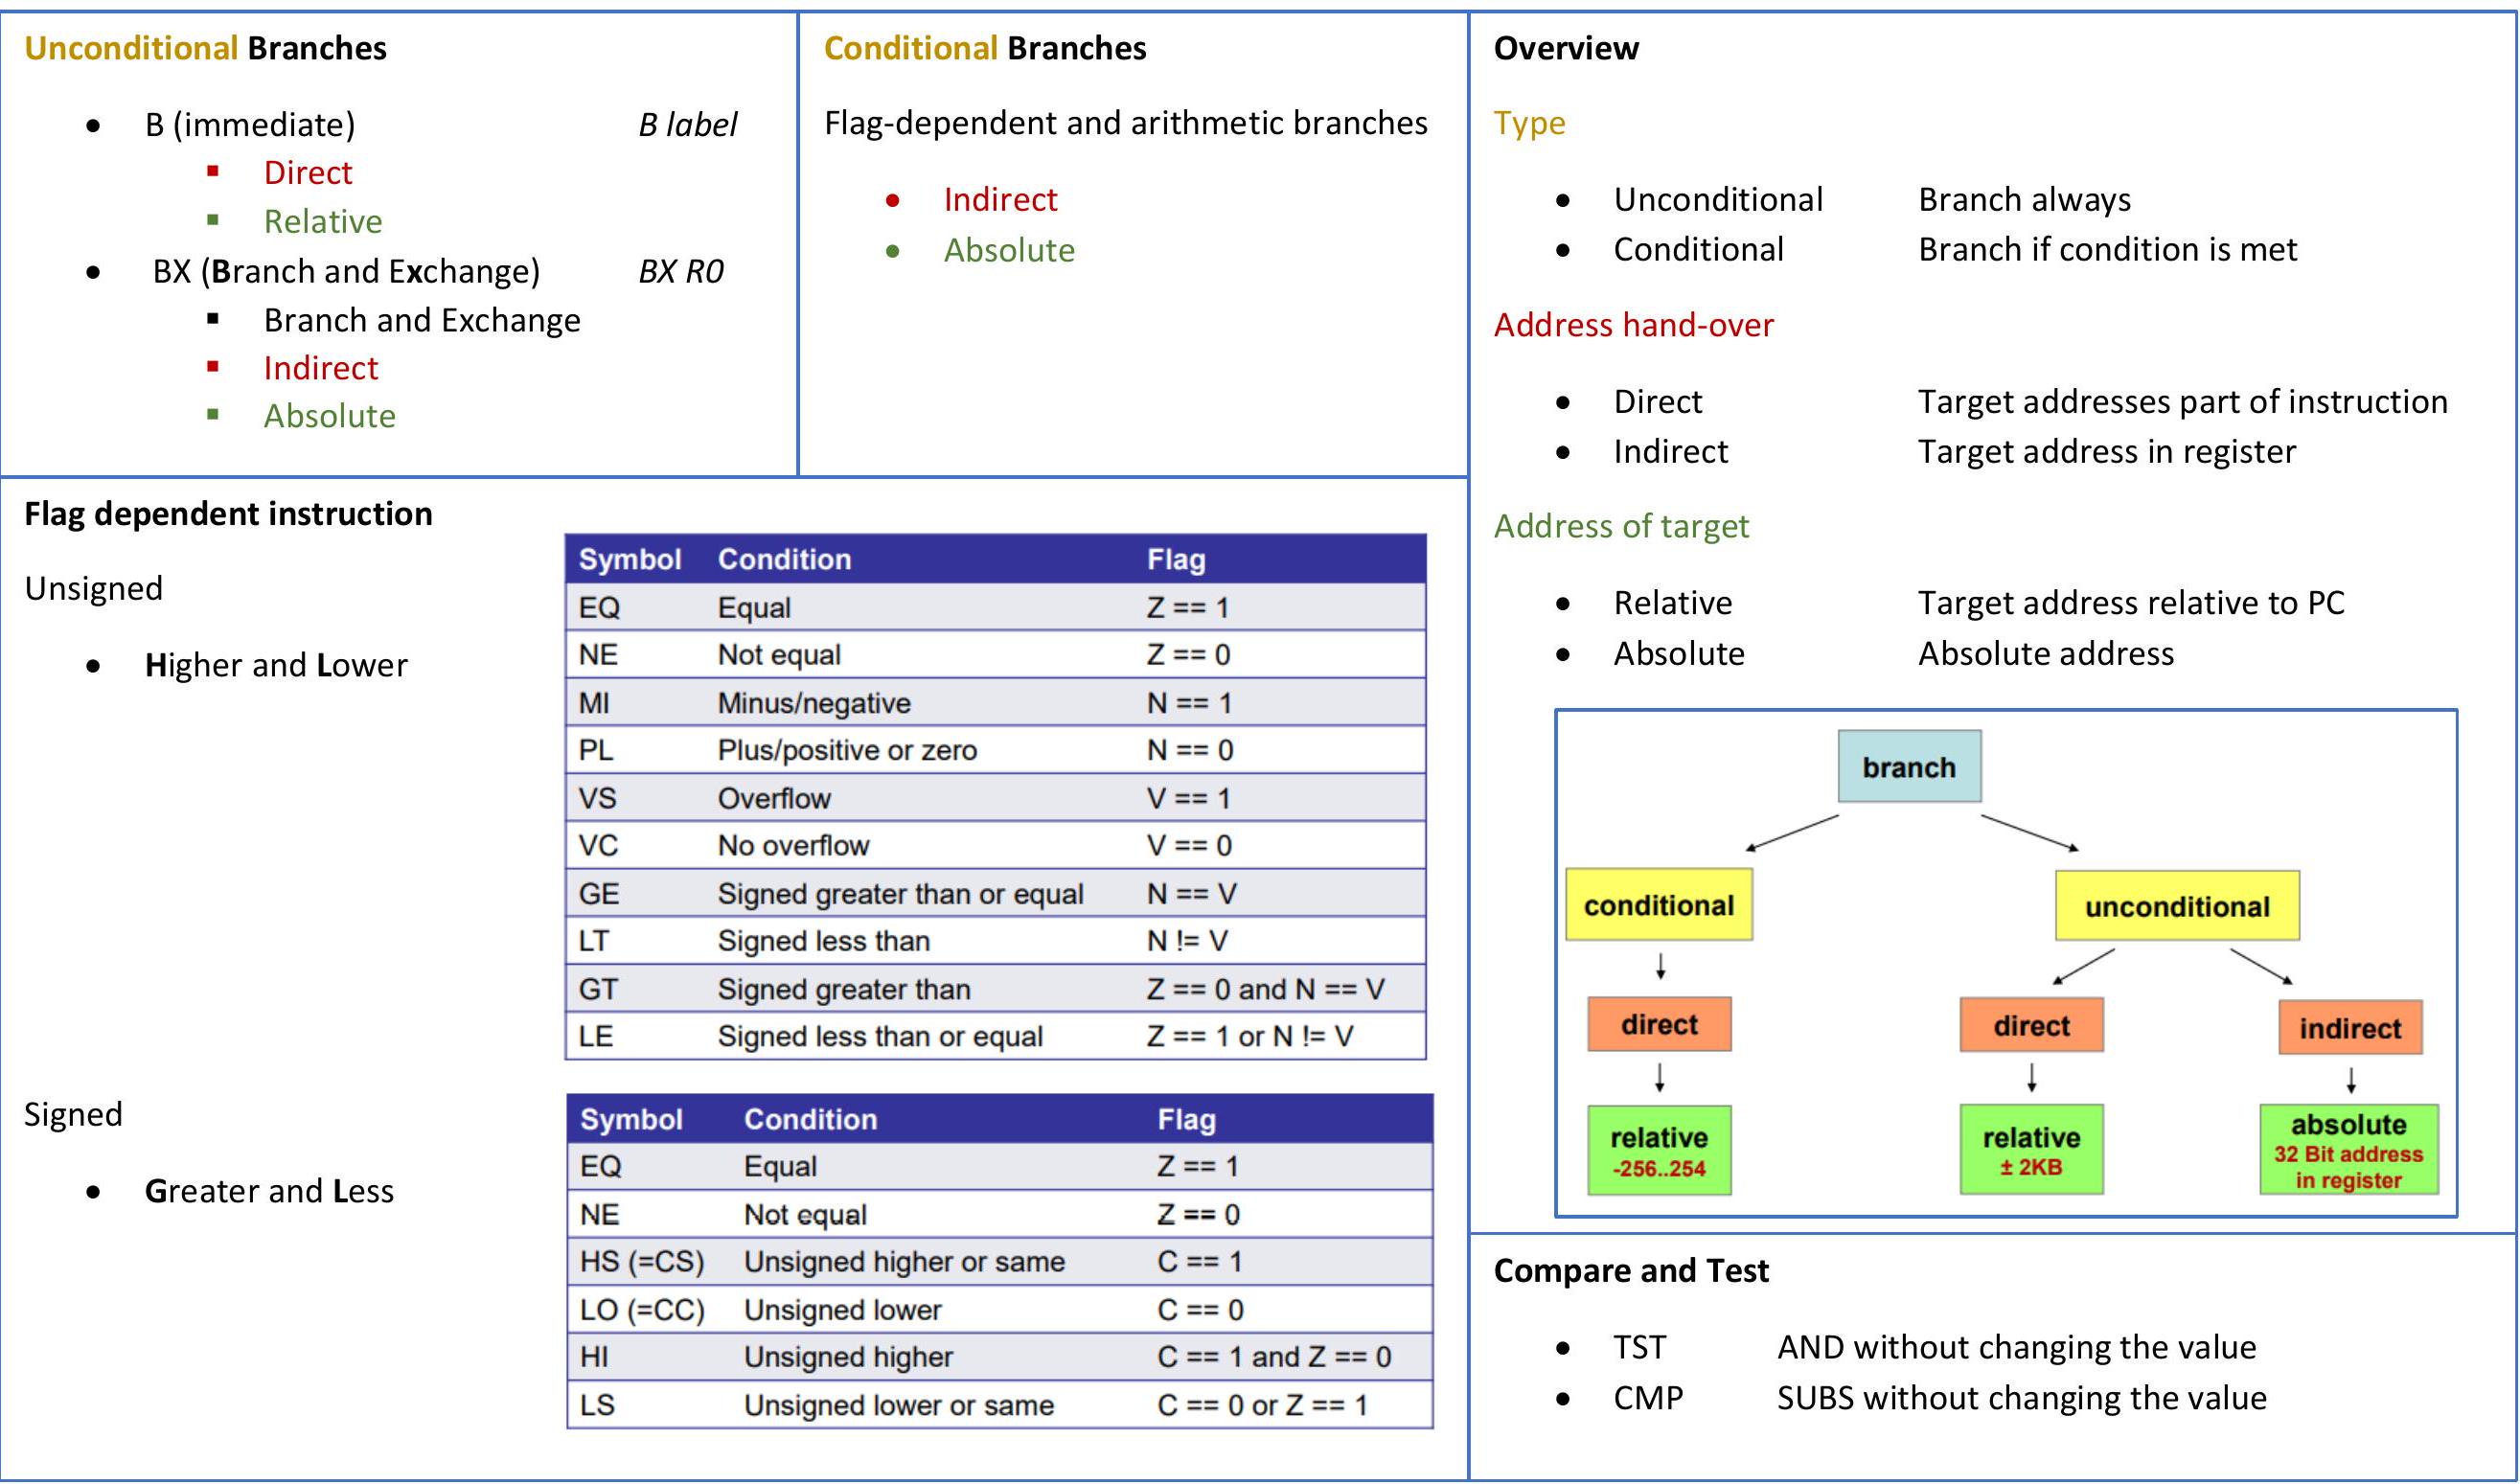
\includegraphics[width=\linewidth]{images/2024_12_29_79e6b22f503fb7b4f718g-05}
\end{center}

\begin{center}
    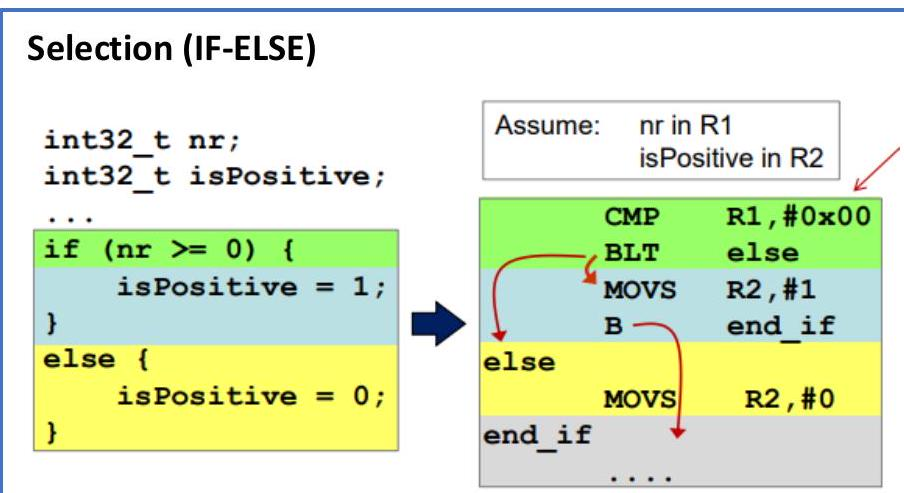
\includegraphics[width=\linewidth]{images/2024_12_29_79e6b22f503fb7b4f718g-07(3)}
    \end{center}
    
    \section*{Switch}
    \section*{- Jump Table}
    uint32\_t result, n; switch (n) 1\\
    case 0:\\
    result += 17; break;\\
    case 1:\\
    result += 13; //fall through\\
    case 3: case 5 result += 37; break;\\
    default:\\
    result $=0$;\\
    \}
    
    \begin{center}
    \begin{tabular}{|c|c|c|}
    \hline
    \multirow[t]{7}{*}{NR\_CASES case\_switch} & EQU & 6 \\
    \hline
     & CMP & R1, \#NR\_CASES \\
    \hline
     & BHS & case\_default \\
    \hline
     & LSLS & R1, \#2 ; * 4 \\
    \hline
     & LDR & R7, =jump\_table \\
    \hline
     & LDR & R7, [R7, R1] \\
    \hline
     & BX & R7 \\
    \hline
    case\_0 & ADDS & R2, R2, \#17 \\
    \hline
    case\_1 & ADDS & R2, R2, \#13 \\
    \hline
    \multirow[t]{2}{*}{case\_3\_5} & ADDS & R2, R2, \#37 \\
    \hline
     & B & end\_sw\_case \\
    \hline
    case\_default & Movs & R2,\#0 \\
    \hline
    end\_sw\_case & ... &  \\
    \hline
    \multirow[t]{6}{*}{jump\_table} & DCD & case\_0 \\
    \hline
     & DCD & case\_1 \\
    \hline
     & DCD & case\_default \\
    \hline
     & DCD & case\_3\_5 \\
    \hline
     & DCD & case\_default \\
    \hline
     & DCD & case\_3\_5 \\
    \hline
    \end{tabular}
    \end{center}
    
    \section*{Loops}
    \begin{itemize}
      \item Do while: Post-Test Loop\\
    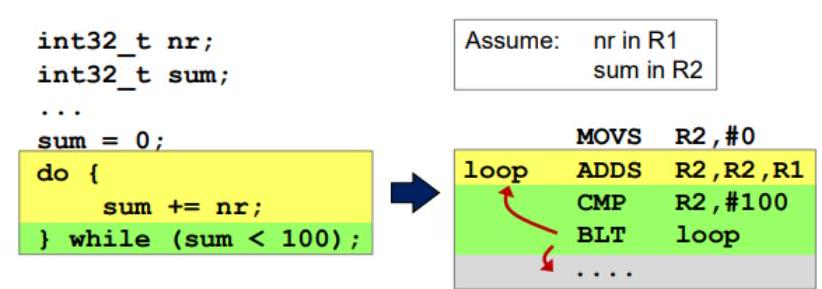
\includegraphics[width=\linewidth]{images/2024_12_29_79e6b22f503fb7b4f718g-07}
      \item While = Pre-Test Loop\\
    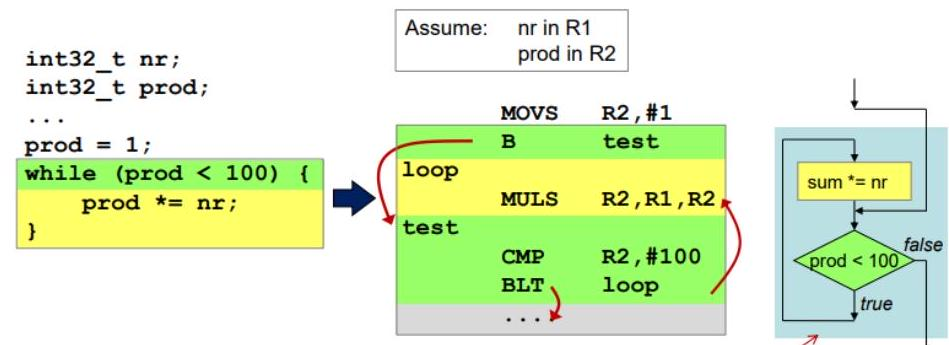
\includegraphics[width=\linewidth]{images/2024_12_29_79e6b22f503fb7b4f718g-07(1)}
      \item For = Pre-Test Loop\\
    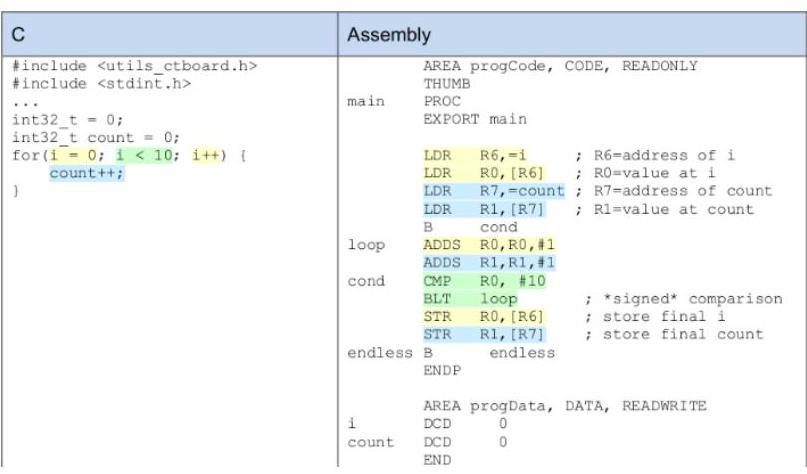
\includegraphics[width=\linewidth]{images/2024_12_29_79e6b22f503fb7b4f718g-07(2)}
    \end{itemize}